
\chapter{\elemMatDetIITitle}\label{elementarydeterminantsII}

In section~\ref{elementarydeterminants}, we saw the definition of the determinant and derived an elementary matrix that exchanges two rows of a matrix.  Next, we need to find elementary matrices corresponding to the other two row operations; multiplying a row by a scalar, and adding a multiple of one row to another.  As a consequence, we will derive some important properties of the determinant.

Consider $M=\colvec{R^1 \\ \vdots \\ R^n }$, where $R^i$ are row vectors.  Let $R^i(\lambda)$ be the identity matrix, with the $i$th diagonal entry replaced by $\lambda$, not to be confused with the row vectors. {\itshape I.e.}
\[
R^i(\lambda)=
\begin{pmatrix}
1 & & & & \\
  & \ddots & & & \\
  & & \lambda & & \\
  & & & \ddots & \\
  & & & & 1 \\
\end{pmatrix}
\, .\]
Then:

\[
M'=R^i(\lambda)M=\colvec{R^1 \\ \vdots \\ \lambda R^i \\ \vdots \\ R^n }
\]
What effect does multiplication by $R^i(\lambda)$ have on the determinant?

\begin{align*}
\det M' & = \sum_{\sigma} \text{sgn}(\sigma) m^1_{\sigma(1)}\cdots \lambda m^i_{\sigma(i)} \cdots m^n_{\sigma(n)} \\
& = \lambda \sum_{\sigma} \text{sgn}(\sigma) m^1_{\sigma(1)}\cdots m^i_{\sigma(i)} \cdots m^n_{\sigma(n)} \\
& = \lambda \det M
\end{align*}
Thus, multiplying a row by $\lambda$ multiplies the determinant by $\lambda$.
{\itshape I.e.,} \[\det R^i(\lambda) M = \lambda \det M\, .\]


\begin{figure}
\begin{center}
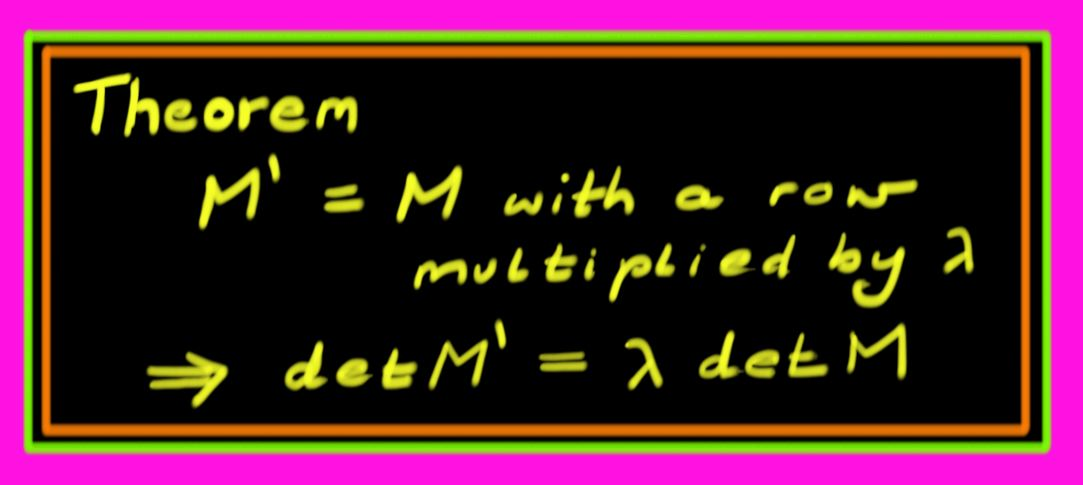
\includegraphics[scale=.27]{\elemMatDetIIPath/row_mult_thm.jpg}
\end{center}
\end{figure}


Since $R^i(\lambda)$ is just the identity matrix with a single row multiplied by $\lambda$, then by the above rule, the determinant of $R^i(\lambda)$ is $\lambda$.  Thus:

\[
\det R^i(\lambda) = \det \begin{pmatrix}
1 & & & & \\
  & \ddots & & & \\
  & & \lambda & & \\
  & & & \ddots & \\
  & & & & 1 \\
\end{pmatrix} = \lambda
\]

The final row operation is adding $\lambda R^j$ to $R^i$.  This is done with the matrix~$S^i_j(\lambda)$, which is an identity matrix but with a $\lambda$ in the $i,j$ position.

\[
S^i_j(\lambda) = \begin{pmatrix}
1 & 	& 	& 	& & & 	\\
  & \ddots & 	&	& & &	\\
  & 	& 1 	& 	& \lambda & &	\\
  & 	& 	& \ddots & & &	\\
  & 	& 	& 	& 1 & & 	\\
  & 	& 	& 	& 	& \ddots & 	\\
  & 	& 	& 	& 	& 	 & 1	\\
\end{pmatrix}
\]
Then multiplying $S^i_j(\lambda)$ by $M$ gives the following:

\[
\begin{pmatrix}
1 & 	& 	& 	& & & 	\\
  & \ddots & 	&	& & &	\\
  & 	& 1 	& 	& \lambda & &	\\
  & 	& 	& \ddots & & &	\\
  & 	& 	& 	& 1 & & 	\\
  & 	& 	& 	& 	& \ddots & 	\\
  & 	& 	& 	& 	& 	 & 1	\\
\end{pmatrix}\colvec{\\ \vdots \\ R^i \\ \vdots \\ R^j \\ \vdots\\ \\}
=
\colvec{\\ \vdots \\ R^i +\lambda R^j \\ \vdots \\ R^j \\ \vdots\\ \\ }
\]
What is the effect of multiplying by $S^i_j(\lambda)$ on the determinant?  Let $M'=S^i_j(\lambda)M$, and let $M''$ be the matrix $M$ but with $R^i$ replaced by $R^j$.

\begin{align*}
\det M' & = \sum_{\sigma} \text{sgn}(\sigma) m^1_{\sigma(1)}\cdots (m^i_{\sigma(i)}+ \lambda m^j_{\sigma(j)}) \cdots m^n_{\sigma(n)} \\
& = \sum_{\sigma} \text{sgn}(\sigma) m^1_{\sigma(1)}\cdots m^i_{\sigma(i)} \cdots m^n_{\sigma(n)} \\
&   \qquad + \sum_{\sigma} \text{sgn}(\sigma) m^1_{\sigma(1)}\cdots \lambda m^j_{\sigma(j)} \cdots m^j_{\sigma(j)} \cdots m^n_{\sigma(n)} \\
& = \det M + \lambda \det M''
\end{align*}
Since $M''$ has two identical rows, its determinant is $0$.  Then \[\det S^i_j(\lambda)M = \det M\, .\]
Notice that if $M$ is the identity matrix, then we have \[\det S^i_j(\lambda) = \det (S^i_j(\lambda)I) = \det I = 1\, .\]

\begin{figure}
\begin{center}
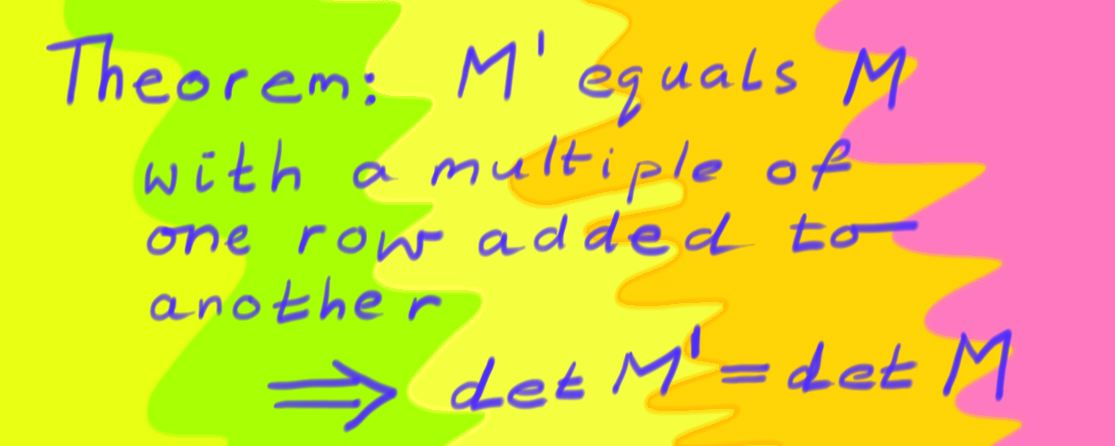
\includegraphics[scale=.27]{\elemMatDetIIPath/row_addition_thm.jpg}
\end{center}
\end{figure}

We now have elementary matrices associated to each of the row operations.

\[
\begin{array}{cccc}
E^i_j &=& I \text{ with rows $i,j$ swapped;} &\det E^i_j=-1 \\[3mm]
R^i(\lambda) &=& I \text{ with $\lambda$ in position $i,i$;} 
	&\det R^i(\lambda)=\lambda \\[3mm]
S^i_j(\lambda) &=& I \text{ with $\lambda$ in position $i,j$;} 
	&\det S^i_j(\lambda)=1 \\[3mm]
\end{array}
\]
\videoscriptlink{elementary_matrices_and_determinants_ii_dets.mp4}{Elementary Determinants}{scripts_elementary_matrices_determinants_ii_dets}
We have also proved the following theorem along the way:

\begin{theorem}
If $E$ is \emph{any} of the elementary matrices $E^i_j, R^i(\lambda), S^i_j(\lambda)$, then $\det(EM)=\det E \det M$.
\end{theorem}

%\href{\webworkurl ReadingHomework13/1/}{Reading homework: problem 13.1}
\reading{13}{1}


\begin{center}
\hspace{3mm}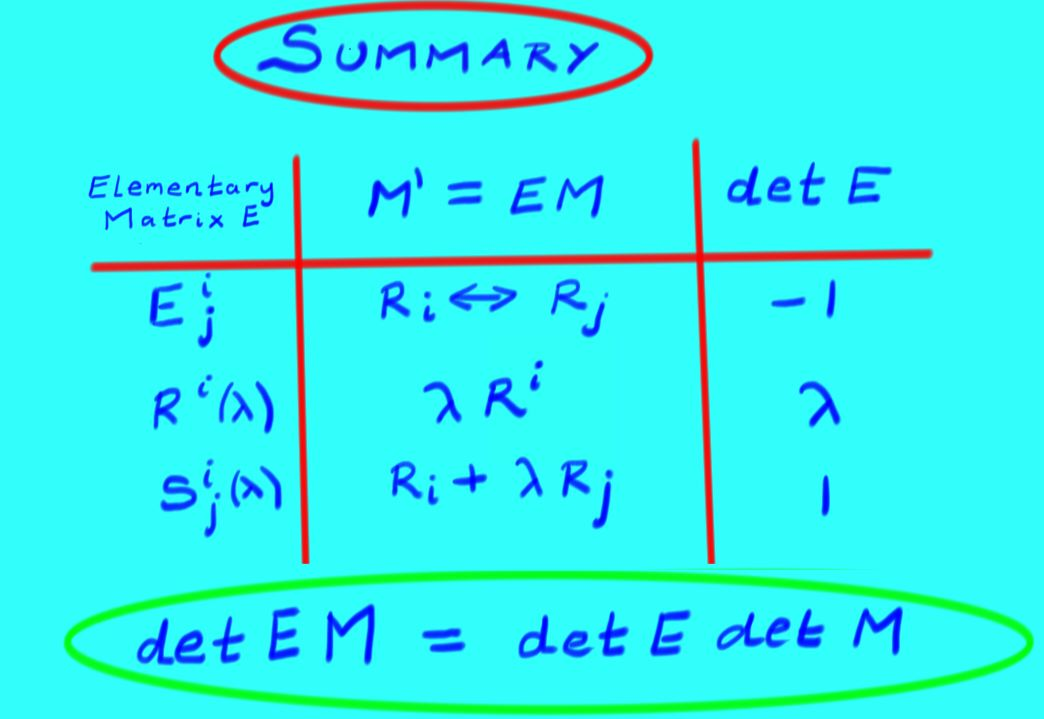
\includegraphics[scale=.27]{\elemMatDetIIPath/summary.jpg}
\end{center}


We have seen that any matrix $M$ can be put into reduced row echelon form via a sequence of row operations, and we have seen that any row operation can be emulated with left matrix multiplication by an elementary matrix.  Suppose that $\rref(M)$ is the reduced row echelon form of $M$.  Then $\rref(M)=E_1E_2\cdots E_kM$ where each $E_i$ is an elementary matrix.

What is the determinant of a square matrix in reduced row echelon form?  
\begin{itemize}
\item If $M$ is not invertible, then some row of $\rref(M)$ contains only zeros.  Then we can multiply the zero row by any constant $\lambda$ without changing~$M$; by our previous observation, this scales the determinant of $M$ by $\lambda$.  Thus, if $M$ is not invertible, $\det \rref(M)=\lambda \det \rref(M)$, and so $\det \rref(M)=0$.  

\item Otherwise, every row of $\rref(M)$ has a pivot on the diagonal; since $M$ is square, this means that $\rref(M)$ is the identity matrix.  Then if $M$ is invertible, $\det \rref(M)=1$.

\item Additionally, notice that $\det \rref(M) = \det (E_1E_2\cdots E_kM)$.  Then by the theorem above, $\det \rref(M)=\det (E_1) \cdots \det (E_k) \det M$.  Since each $E_i$ has non-zero determinant, then $\det \rref(M)=0$ if and only if $\det M=0$.
\end{itemize}
Then we have shown:

\begin{theorem}
\label{detinvertible}
For any square matrix $M$, $\det M\neq 0$ if and only if $M$ is invertible.
\end{theorem}
Since we know the determinants of the elementary matrices, we can immediately obtain the following:


\videoscriptlink{elementary_matrices_ii_inverses_determinants.mp4}{Determinants and Inverses}{scripts_elementary_matrices_determinants_ii_inverses}

\begin{figure}
\begin{center}
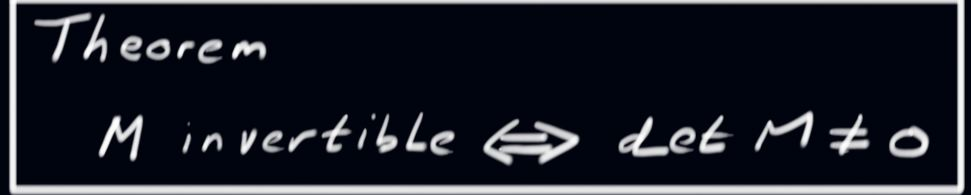
\includegraphics[scale=.27]{\elemMatDetIIPath/theorem_invertible.jpg}
\end{center}
\end{figure}

\begin{corollary}
Any elementary matrix $E^i_j, R^i(\lambda), S^i_j(\lambda)$ is invertible, except for $R^i(0)$.  In fact, the inverse of an elementary matrix is another elementary matrix.
\end{corollary}


To obtain one last important result, suppose that $M$ and $N$ are square $n\times n$ matrices, with reduced row echelon forms such that, for elementary matrices  $E_i$ and $F_i$, \[M=E_1E_2\cdots E_k \, \rref(M)\, ,\] and  \[N=F_1F_2\cdots F_l \, \rref(N)\, .\]  If $\rref(M)$ is the identity matrix ({\itshape i.e.}, $M$ is invertible), then:

\begin{align*}
\det (MN) & = \det (E_1E_2\cdots E_k\,  \rref(M) F_1F_2\cdots F_l \, \rref(N) )\\
& = \det (E_1E_2\cdots E_k I F_1F_2\cdots F_l\,  \rref(N) )\\
& = \det (E_1) \cdots \det(E_k)\det(I)\det(F_1)\cdots\det(F_l)\det(\rref(N)\\
& = \det(M)\det(N)
\end{align*}
Otherwise, $M$ is not invertible, and $\det M=0=\det 
\rref(M)$.  Then there exists a row of zeros in $
\rref(M)$, so $R^n(\lambda)
\rref(M)=
\rref(M)$.  Then:
\begin{align*}
\det (MN)
& = \det (E_1E_2\cdots E_k \, \rref(M) N )\\
& = \det (E_1E_2\cdots E_k \, \rref(M) N )\\
& = \det (E_1) \cdots \det(E_k)\det( \rref(M)N)\\
& = \det (E_1) \cdots \det(E_k)\det( R^n(\lambda) \, \rref(M)N)\\
& = \det (E_1) \cdots \det(E_k)\lambda \det( \rref(M)N)\\
& = \lambda \det (MN)
\end{align*}
Which implies that $\det (MN)=0=\det M \det N$.

Thus we have shown that for {\itshape any} matrices $M$ and $N$, 
\label{detmultiplicative}
\[
\det (MN) = \det M \det N
\]
This result is {\itshape extremely important}; do not forget it!

\videoscriptlink{elementary_matrices_determinant_ii_product.mp4}{Alternative proof}{scripts_elementary_matrices_determinants_ii_product}

\begin{figure}
\begin{center}

\includegraphics[scale=.27]{\elemMatDetIIPath/detMN.jpg}
\end{center}
\end{figure}

%\href{\webworkurl ReadingHomework13/2/}{Reading homework: problem 13.2}
\reading{13}{2}

%\section*{References}
%Hefferon, Chapter Four, Section I.1 and I.3
%\\
%Beezer, Chapter D, Section DM, Subsection EM
%\\
%Beezer, Chapter D, Section PDM
%\\
%Wikipedia:
%\begin{itemize}
%\item \href{http://en.wikipedia.org/wiki/Determinant}{Determinant}
%\item \href{http://en.wikipedia.org/wiki/Elementary_matrix}{Elementary Matrix}
%\end{itemize}

\section{Review Problems}





\begin{enumerate}
\item \label{det33} Let $M=\begin{pmatrix}
m^1_1 & m^1_2 & m^1_3\\
m^2_1 & m^2_2 & m^2_3\\
m^3_1 & m^3_2 & m^3_3\\
\end{pmatrix}$.  Use row operations to put $M$ into \emph{row echelon form}.  For simplicity, assume that $m_1^1\neq 0 \neq m^1_1m^2_2-m^2_1m^1_2$.

Prove that $M$ is non-singular if and only if:
\[
m^1_1m^2_2m^3_3 
- m^1_1m^2_3m^3_2 
+ m^1_2m^2_3m^3_1 
- m^1_2m^2_1m^3_3 
+ m^1_3m^2_1m^3_2
- m^1_3m^2_2m^3_1
\neq 0
\]

\phantomnewpage

\item 
\begin{enumerate}
\item What does the matrix $E^1_2=\begin{pmatrix}
0 & 1 \\
1 & 0
\end{pmatrix}$ do to $M=\begin{pmatrix}
a & b \\
d & c
\end{pmatrix}$ under left multiplication?  What about right multiplication?
\item Find elementary matrices $R^1(\lambda)$ and $R^2(\lambda)$ that respectively multiply rows $1$ and $2$ of $M$ by $\lambda$ but otherwise leave $M$ the same under left multiplication.
\item Find a matrix $S^1_2(\lambda)$ that adds a multiple $\lambda$ of row $2$ to row $1$ under left multiplication.
\end{enumerate}

\phantomnewpage

\item Let $M$ be a matrix and $S^i_jM$ the same matrix with rows \(i\) and \(j\) switched.  Explain every line of the 
\hyperlink{rowswap}{series of equations} proving that $\det M = -\det (S^i_jM)$.

\phantomnewpage

%\item \label{prob_inversion_number} This problem is a ``hands-on'' look at why \hyperlink{permutation_parity}{the property} describing the parity of permutations is true.
%
%\hypertarget{inversion_number}{The \emph{inversion number}}\index{Permutation!Inversion number} of a permutation $\sigma$ is the number of pairs $i<j$ such that $\sigma(i)>\sigma(j)$; it's the number of ``numbers that appear left of smaller numbers'' in the permutation.  For example, for the permutation $\rho = [4,2,3,1]$, the inversion number is $5$. The number $4$ comes before $2,3,$ and $1$, and $2$ and $3$ both come before $1$.
%
%Given a permutation $\sigma$, we can make a new permutation $\tau_{i,j} \sigma$ by exchanging the $i$th and $j$th entries of $\sigma$.
%
%\begin{enumerate}
%\item What is the inversion number of the permutation \(\mu=[1,2,4,3]\) that exchanges 4 and 3 and leaves everything else alone? Is it an even or an odd permutation?
%
%\item What is the inversion number of the permutation \(\rho=[4,2,3,1]\) that exchanges 1 and 4 and leaves everything else alone? Is it an even or an odd permutation?
%
%\item What is the inversion number of the permutation \(\tau_{1,3} \mu\)? Compare the parity\footnote{The \emph{parity} of an integer refers to whether the integer is even or odd. Here the parity of a permutation $\mu$ refers to the parity of its inversion number.} of \(\mu\) to the parity of \(\tau_{1,3} \mu.\)
%
%\item What is the inversion number of the permutation \(\tau_{2,4} \rho\)? Compare the parity of \(\rho\) to the parity of \(\tau_{2,4} \rho.\)
%
%\item What is the inversion number of the permutation \(\tau_{3,4} \rho\)? Compare the parity of \(\rho\) to the parity of \(\tau_{3,4} \rho.\)
%\end{enumerate}
%
%\videoscriptlink{elementary_matrices_determinant_hint.mp4}{Problem~\ref{prob_inversion_number} hints}{scripts_elementary_matrices_determinants_hint}

\phantomnewpage

%\item \label{problem_permutation} (Extra credit) Here we will examine a (very) small set of the general properties about permutations and their applications. In particular, we will show that one way to compute the sign of a permutation is by finding the \hyperlink{inversion_number}{inversion number} $N$ of $\sigma$ and we have
%\[
%\sgn(\sigma) = (-1)^N.
%\]
%
%For this problem, let $\mu = [1,2,4,3]$.
%
%\begin{enumerate}
%\item Show that every permutation $\sigma$ can be sorted by only taking simple (adjacent) transpositions\index{Permutation!Simple transposition} $s_i$ where $s_i$ interchanges the numbers in position $i$ and $i+1$ of a permutation $\sigma$ (in our other notation $s_i = \tau_{i,i+1}$). For example $s_2 \mu = [1, 4, 2, 3]$, and to sort $\mu$ we have $s_3 \mu = [1, 2, 3, 4]$.
%
%\item \label{prob_part_relations} We can compose simple transpositions together to represent a permutation (note that the sequence of compositions is not unique), and these are associative, we have an identity (the trivial permutation where the list is in order or we do nothing on our list), and we have an inverse since it is clear that $s_i s_i \sigma = \sigma$. Thus permutations of $[n]$ under composition are an example of a \hyperref[groups]{group}. However note that not all simple transpositions commute with each other since
%\begin{align*}
%s_1 s_2 [1, 2, 3] & = s_1 [1, 3, 2] = [3, 1, 2]
%\\ s_2 s_1 [1, 2, 3] & = s_2 [2, 1, 3] = [2, 3, 1]
%\end{align*}
%(you will prove here when simple transpositions commute). When we consider our initial permutation to be the trivial permutation $e = [1, 2, \dotsc, n]$, we do not write it; for example $s_i \equiv s_i e$ and $\mu = s_3 \equiv s_3 e$. This is analogous to not writing 1 when multiplying. Show that $s_i s_i = e$ (in shorthand $s_i^2 = e$), $s_{i+1} s_i s_{i+1} = s_i s_{i+1} s_i$ for all $i$, and $s_i$ and $s_j$ commute for all $|i - j| \geq 2$.
%
%\item Show that every way of expressing $\sigma$ can be obtained from using the relations proved in part~\ref{prob_part_relations}. In other words, show that for any expression $w$ of simple transpositions representing the trivial permutation $e$, using the proved relations.
%
%\emph{Hint: Use induction on $n$. For the induction step, follow the path of the $(n+1)$-th strand by looking at $s_n s_{n-1} \cdots s_k s_{k\pm1} \cdots s_n$ and argue why you can write this as a subexpression for any expression of $e$. Consider using diagrams of these paths to help.}
%
%\item The simple transpositions \hyperlink{action}{acts on} an $n$-dimensional vector space $V$ by $s_i v = E^i_{i+1} v$ (where $E^i_j$ is \hyperlink{elem_matrix_row_swap}{an elementary matrix}) for all vectors $v \in V$. Therefore we can just represent a permutation $\sigma$ as the matrix $M_{\sigma}$\footnote{Often people will just use $\sigma$ for the matrix when the context is clear.}, and we have $\det(M_{s_i}) = \det(E^i_{i+1}) = -1$. Thus prove that $\det(M_{\sigma}) = (-1)^N$ where $N$ is a number of simple transpositions needed to represent $\sigma$ as a permutation. You can assume that $M_{s_i s_j} = M_{s_i} M_{s_j}$ (it is not hard to prove) and that $\det(A B) = \det(A) \det(B)$ \hyperref[detmultiplicative]{from Chapter~\ref*{elementarydeterminantsII}}.
%
%\emph{Hint: You to make sure $\det(M_{\sigma})$ is well-defined since there are infinite ways to represent $\sigma$ as simple transpositions.}
%
%\item Show that $s_{i+1} s_i s_{i+1} = \tau_{i, i+2}$, and so give one way of writing $\tau_{i, j}$ in terms of simple transpositions? Is $\tau_{i,j}$ an even or an odd permutation? What is $\det(M_{\tau_{i,j}})$? What is the inversion number of $\tau_{i,j}$?
%
%\item The minimal number of simple transpositions needed to express $\sigma$ is called the \emph{length}\index{Permutation!Length} of $\sigma$; for example the length of $\mu$ is 1 since $\mu = s_3$. Show that the length of $\sigma$ is equal to the inversion number of $\sigma$.
%
%\emph{Hint: Find an procedure which gives you a new permutation $\sigma^{\prime}$ where $\sigma = s_i \sigma^{\prime}$ for some $i$ and the inversion number for $\sigma^{\prime}$ is 1 less than the inversion number for $\sigma$.}
%
%\item Show that $(-1)^N = \sgn(\sigma) = \det(M_{\sigma})$, where $\sigma$ is a permutation with $N$ inversions. Note that this immediately implies that $\sgn(\sigma \rho) = \sgn(\sigma) \sgn(\rho)$ for any permutations $\sigma$ and $\rho$.
%\end{enumerate}

\item Let $M'$ be the matrix obtained from $M$ by swapping two columns $i$ and $j$. Show that $\det M'=-\det M $.

\item The scalar triple product of three vectors $u,v,w$ from $\Re^3$ is $u\cdot(v\times w)$. Show that this product is the same as the determinant of the matrix whose columns are $u,v,w$ (in that order). What happens to the scalar triple product when the factors are permuted? 

\item Show that if $M$ is a $3\times 3$ matrix whose third row is a sum of multiples of the other rows ($R_3=aR_2+bR_1$) then $\det M=0$. Show that the same is true if one of the columns is a sum of multiples of the others. 

\end{enumerate}

\phantomnewpage

\newpage



